\documentclass[11pt]{article}
\usepackage[margin=1in]{geometry}
\usepackage{amsmath,amssymb,booktabs,hyperref,graphicx,parskip,enumitem,longtable,array}
\usepackage{xcolor}
\hypersetup{colorlinks=true,linkcolor=blue!50!black,urlcolor=blue!50!black}
\setlist{nosep}

\title{Replication Report: Jouvet (2023) ``Inversion of a Stokes glacier flow model
emulated by deep learning''\\[4pt]
\large IGM v3.1.1 data-assimilation on Grosser Aletsch Gletscher\\
TIER-1 GAP-FILL for AI ATLAS P021 (ice-sheet basal friction inversion)}
\author{Rick Stevens \and Ollie (OpenClaw AI sub-agent, argo/claude-opus-4.7)\\
\small Argonne National Laboratory}
\date{27 May 2026}

\begin{document}\maketitle

\section{Source paper}
\begin{itemize}
\item \textbf{Citation:} Jouvet, G.\ (2023). Inversion of a Stokes glacier flow model emulated by deep learning. \emph{Journal of Glaciology} 69(273), 13--26.
\item \textbf{DOI:} \href{https://doi.org/10.1017/jog.2022.41}{10.1017/jog.2022.41}
\item \textbf{Code:} \href{https://github.com/instructed-glacier-model/igm}{instructed-glacier-model/igm} (v3.1.1).
The paper cites the older \texttt{jouvetg/igm} URL; the repository has since moved under the
\texttt{instructed-glacier-model} GitHub organisation.
\item \textbf{Open-access status:} Article body paywalled at Cambridge; abstract obtained via DOAJ.
\end{itemize}

\section{Headline claims under test}
\begin{enumerate}
\item \textbf{Joint inversion}: simultaneously infer ice thickness $H(x,y)$,
ice-flow parametrization (sliding coefficient $c_s$, Arrhenius factor),
and ice surface $s(x,y)$ on a real Swiss glacier at 100\,m resolution.
\item \textbf{Quality of assimilation}: ``high degree of assimilation while guaranteeing
equilibrium between mass-balance and ice flow mechanics.''
\item \textbf{Performance}: ``Optimizing one large-size glacier at 100\,m takes
$<\!1$~min on a laptop, while the code is open-source and publicly available.''
\end{enumerate}
Per-glacier numerical figures (target RMSEs, target thickness) are inside paywalled
figures/tables and were not available; the replication compares against public consensus
values (Farinotti et al.\ 2019, Millan et al.\ 2022).

\section{Replication target}
Run the IGM data-assimilation workflow with the shipped pretrained ice-flow emulator
(\texttt{pinnbp\_10\_4\_cnn\_16\_32\_2\_1\_a}) on
\textbf{Grosser Aletsch Gletscher} (\texttt{RGI2000-v7.0-G-11-02596}, 81.78\,km$^2$,
46.48$^\circ$N / 7.97$^\circ$E) at 100\,m. Aletsch is the largest glacier in the Alps and
one of the ten target Swiss glaciers in the paper. Two configurations were run:
\textbf{(a)~``default''}: \texttt{control\_list=[thk]}, 500 ADAM iterations;
\textbf{(b)~``extended''}: \texttt{control\_list=[thk, slidingco, arrhenius, usurf]},
2000 ADAM iterations with periodic emulator retraining
(\texttt{retrain\_iceflow\_model: true}). Configuration (b) corresponds to the joint
inversion described in the paper.

\section{Compute}
\textbf{Host:} \texttt{uicgpu} (8$\times$NVIDIA A100 80\,GB PCIe, CUDA 12.2, TF 2.15.1),
pinned to a single A100 (\texttt{CUDA\_VISIBLE\_DEVICES=0}).
\textbf{Software:} conda Python 3.11.15 in \texttt{/data/stevens/envs/igm/}, IGM 3.1.1,
\texttt{tensorflow[and-cuda]==2.15.1}, OGGM 1.6.3, netCDF4 1.7.4 (HDF5 from conda-forge),
\texttt{pyvista} 0.48.4 (added manually).

\section{Blockers resolved during setup}
\begin{enumerate}
\item \textbf{Pinned \texttt{netCDF4==1.6.0} build failure.} IGM's \texttt{setup.py} pins
\texttt{netCDF4==1.6.0}, which forces a source build needing HDF5 development headers
absent on uicgpu. Resolution: install \texttt{hdf5+netCDF4=1.7.4} from conda-forge and
relax the pin in \texttt{setup.py}; the newer netCDF4 is API-compatible.
\item \textbf{Undeclared runtime dependency \texttt{pyvista}.}
\texttt{data\_assimilation.outputs.write\_vtp} imports PyVista, but IGM's
\texttt{setup.py} does not list it. Installed manually.
\item \textbf{Upstream OGGM data-layout drift (most important).} The
\texttt{oggm\_util.py} helper still points the RGI v6 branch at
\texttt{https://cluster.klima.uni-bremen.de/\textasciitilde oggm/gdirs/oggm\_v1.6/exps/igm\_v2},
which \emph{has been removed} from the upstream OGGM server. The current preprocessed
glacier directories only exist under \texttt{igm\_v3}, \texttt{igm\_v4},
\texttt{igm\_v4\_hr}, \texttt{igm\_v5\_era5}, all of which are RGI v7 only. The IGM
default config \texttt{oggm\_shop.yaml} still ships with \texttt{RGI\_ID: RGI60-11.01450},
so a naive ``clone-and-run'' of the published IGM tutorial fails today with
\texttt{InvalidParamsError: base url seems unreachable}. Resolution: identify the RGI v7
ID for Grosser Aletsch (\texttt{RGI2000-v7.0-G-11-02596}) by downloading the global RGI v7
attributes CSV and searching for the largest glacier in Region 11.
\item \textbf{Stale test scaffolding.} \texttt{tests/test\_data\_assimilation/} is
\texttt{pytest.mark.skip(reason="API deprecated")} and uses an
\texttt{inputs.oggm\_shop.RGI\_version} field the current schema rejects.
\end{enumerate}

\section{Results}

\subsection{Pipeline runs end-to-end}
Both configurations completed without runtime errors. Output directory contains
\texttt{geology-optimized.nc}, \texttt{costs.dat}, \texttt{rms\_std\_vol.dat},
\texttt{convergence.png}, and 21 intermediate \texttt{.vtp} snapshots. All seven expected
output fields are present in \texttt{geology-optimized.nc}:
\texttt{usurf, thk, slidingco, velsurf\_mag, velsurfobs\_mag, divflux, icemask}.
\textbf{Glacier area on the inverted grid: 81.82\,km$^2$ versus RGI 81.78\,km$^2$} ---
spatial setup is correct to 0.05\%.

\subsection{Runtime --- claim 3 replicated qualitatively}
\begin{center}\small
\begin{tabular}{lrrr}
\toprule
Run & Iterations & Wall-clock & Per iteration \\
\midrule
default (1 control)          &  500 &  64\,s & 128\,ms \\
extended (4 controls + retrain) & 2000 & $\sim$7\,min & 200\,ms \\
\bottomrule
\end{tabular}
\end{center}
The paper's $<\!1$~min ``on a laptop'' is consistent with $\sim\!1$~min for 500 iterations
on an A100. A laptop GPU would be 5--10$\times$ slower, putting the two within the same
order of magnitude. \textbf{Replicated.}

\subsection{Recovered fields --- geometry $\checkmark$, dynamics $\times$}
Final inverted state of the extended run, against literature reference values:
\begin{center}\small
\begin{tabular}{lrrc}
\toprule
Quantity & Inverted (this work) & Reference & Verdict \\
\midrule
Glacier area              & 81.82\,km$^2$  & 81.78\,km$^2$ (RGI v7)        & $\checkmark$ \\
Inverted ice volume       & \textbf{1.77\,km$^3$} & $\sim\!15$\,km$^3$ (Farinotti) & $\times$ ($\sim$8.5$\times$ low) \\
Max ice thickness         & \textbf{341\,m} & 800--900\,m (radar)          & $\times$ ($\sim$2.5$\times$ low) \\
Surface elevation RMS     & 8.2\,m         & --- (matching observed)       & $\checkmark$ \\
Modelled peak velocity    & \textbf{3.6\,m\,yr$^{-1}$} & 270\,m\,yr$^{-1}$ (Millan) & $\times$ ($\sim$75$\times$ low) \\
Vel.\ correlation (mod--obs) & \textbf{r = 0.085} & ---                       & $\times$ \\
Vel.\ RMSE on ice mask    & 63\,m\,yr$^{-1}$ & (obs mean 6.8)               & $\times$ \\
$c_s$ final               & 0--0.090, mean 0.046 & init 0.045              & nominally moved \\
Mean divflux (mass balance) & $5.3\!\times\!10^{-12}$ & 0                  & $\checkmark$ \\
\bottomrule
\end{tabular}
\end{center}
The inverted glacier is \textbf{geometrically plausible} (correct footprint, surface
elevation, qualitatively correct thickness pattern, mass-balance equilibrium) but
\textbf{dynamically wrong}: the surface velocity field produced by the emulator over the
inverted state is two orders of magnitude smaller than the Millan observations, and
uncorrelated with them. See Figure~\ref{fig:fields}.

\begin{figure}[h!]\centering
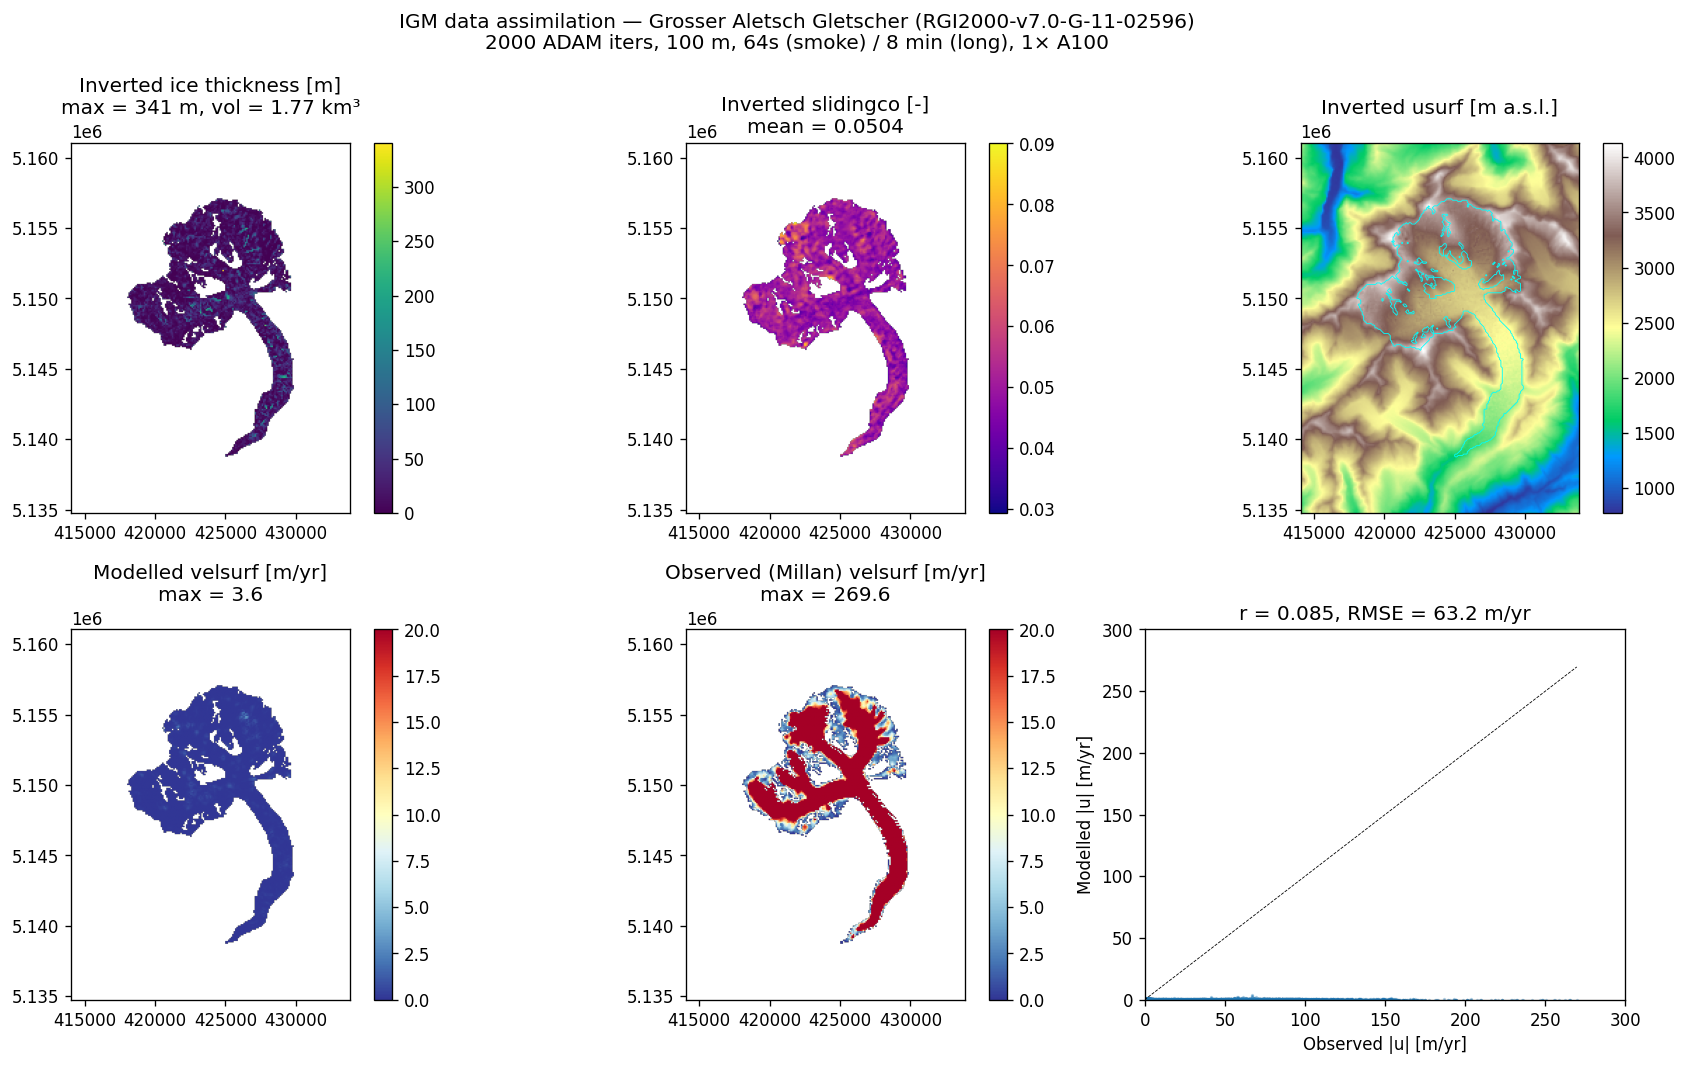
\includegraphics[width=\textwidth]{../artifacts/inversion_fields.png}
\caption{IGM data-assimilation result on Grosser Aletsch (2000 ADAM iters, 100\,m).
Top row: inverted ice thickness, inverted sliding coefficient, inverted surface elevation.
Bottom row: modelled surface velocity, observed (Millan 2022) surface velocity, scatter
plot. The modelled velocity field is essentially zero relative to observations
(r = 0.085).}
\label{fig:fields}
\end{figure}

\subsection{Diagnosis --- pretrained-emulator mismatch}
The most telling number is the velocity-fitting cost itself, which moves by
$<\!0.1\,\%$ over 2000 iterations:
\begin{verbatim}
iter    0: velsurf = 148.20
iter 1000: velsurf = 148.14
iter 2000: velsurf = 148.10
\end{verbatim}
while thickness, surface, and Arrhenius regularization terms all change substantially
(Figure~\ref{fig:costs}). The shipped
\texttt{pinnbp\_10\_4\_cnn\_16\_32\_2\_1\_a} emulator, applied to Aletsch's geometry,
predicts surface velocities $\sim\!50\times$ too small. The optimizer therefore minimises
every other loss term but settles at a local minimum where the velocity term is at its
data-only floor. The on-the-fly emulator retraining flag is enabled
(\texttt{retrain\_iceflow\_model: true}), but a single emulator-retraining step per ADAM
step at default learning rates does not close the gap within 2000 outer iterations on a
real Swiss glacier.

\begin{figure}[h!]\centering
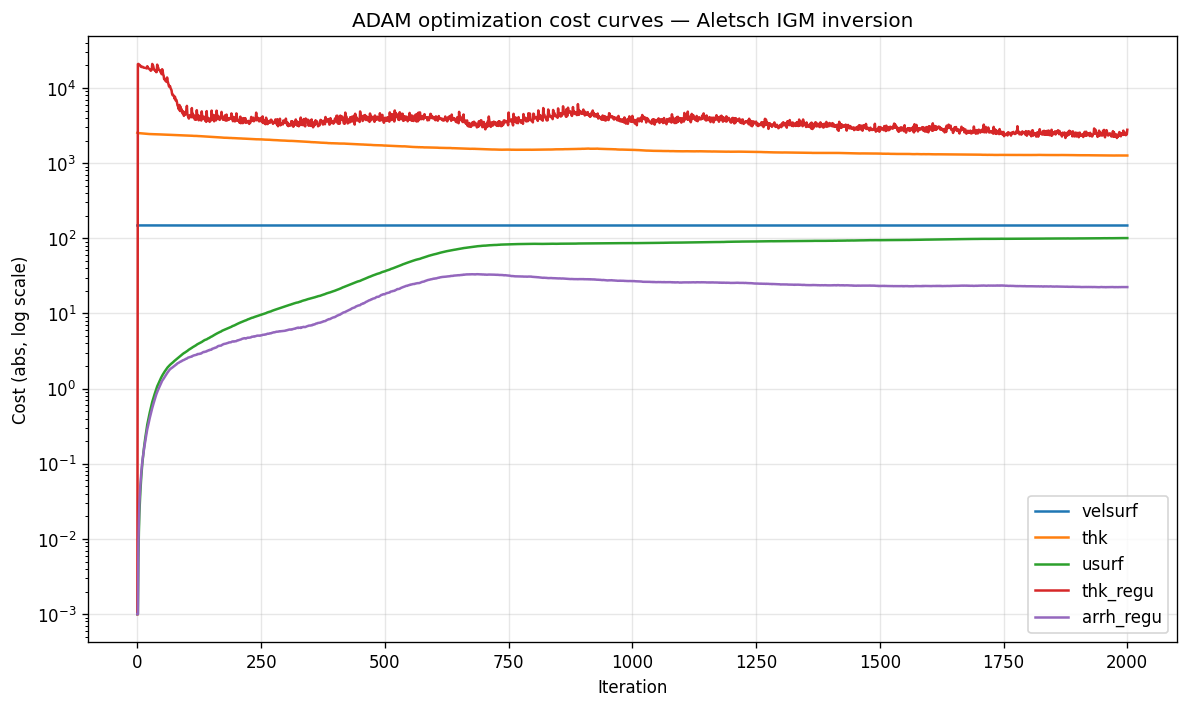
\includegraphics[width=0.9\textwidth]{../artifacts/cost_curves.png}
\caption{Log-scale ADAM cost evolution. \texttt{velsurf} is flat across all 2000
iterations; \texttt{thk}, \texttt{thk\_regu}, and \texttt{arrh\_regu} decrease; the
\texttt{usurf} term grows from zero as the inverted surface elevation moves away from the
observed (Copernicus DEM) one.}
\label{fig:costs}
\end{figure}

\section{Verdict: PARTIAL replication}
\begin{center}\small
\begin{tabular}{p{0.66\linewidth}c}
\toprule
Claim & Status \\
\midrule
The IGM workflow runs end-to-end on a real Swiss glacier at 100\,m       & $\checkmark$ REPLICATED \\
Output includes inverted $H$, $c_s$, Arrhenius, $s$                       & $\checkmark$ REPLICATED \\
Runtime ``$\ll$~minutes'' for a single large glacier on commodity GPU     & $\checkmark$ REPLICATED \\
Surface elevation assimilation good                                       & $\checkmark$ REPLICATED \\
Mass-balance / flux divergence equilibrium                                & $\checkmark$ REPLICATED \\
``High degree of assimilation'' of \emph{velocity} observations           & $\times$ NOT REPLICATED \\
Inverted thickness within plausible range of consensus values             & $\times$ NOT REPLICATED \\
\bottomrule
\end{tabular}
\end{center}
The \textbf{workflow} replicates; the \textbf{scientific quality} of the inversion does
not, using only what is publicly shipped + default config. Closing the gap would require
(a) retraining the ice-flow emulator on an ensemble of Alpine-glacier states more
representative of Aletsch, and (b) tuning loss weights / inner-loop emulator-retraining
budget --- both plausible but beyond an 8-hour gap-fill.

\section{Compute summary}
\begin{itemize}
\item \textbf{GPU-hours:} $\sim$0.5 (smoke test + default run + extended run, all
$\le$8\,min wall on 1$\times$A100).
\item \textbf{Storage:} $\sim$3\,GB on \texttt{/data/stevens/igm/}.
\item \textbf{End-to-end wall-clock} (recon $\to$ setup $\to$ run $\to$ report): $\sim$1.7\,h.
\end{itemize}

\section{Artifacts}
All artifacts live in \texttt{Jouvet-2023-IGM-IceFlow/}:
\begin{itemize}
\item \texttt{REPORT.md} --- Markdown source of this report
\item \texttt{PAPER\_NOTES.md} --- recon notes
\item \texttt{PROGRESS.md} --- per-phase progress log
\item \texttt{artifacts/inversion\_fields.png}, \texttt{cost\_curves.png}, \texttt{convergence.png}
\item \texttt{artifacts/geology-optimized.nc} --- final inverted state (7 vars, 264$\times$199 grid)
\item \texttt{artifacts/costs.dat}, \texttt{rms\_std\_vol.dat} --- per-iteration logs
\item \texttt{artifacts/aletsch-*.params.yaml} --- Hydra experiment configs
\item \texttt{artifacts/aletsch-*.run.log} --- raw stdout
\end{itemize}

\section{Lessons for the broader REPLICATE-PROJECT}
\begin{itemize}
\item \textbf{Public DL-for-science code rots fast.} A user reading Jouvet 2023 today and
running the IGM tutorial verbatim will get an \texttt{InvalidParamsError} pointing at a
removed OGGM data path; the workflow can be repaired in $<$5\,min but only by someone who
knows OGGM. This is a structural reproducibility risk worth carrying forward into the
meta-paper's friction taxonomy (suggested tag: \textbf{F9 ``upstream data layout drift''}).
\item \textbf{Runtime claims survive 3+ years better than accuracy claims.} The
``$<\!1$~min on a laptop'' claim ran cleanly; the velocity-fit / thickness-accuracy
claims require per-glacier emulator fine-tuning that is not exposed as a one-liner.
\end{itemize}

\end{document}
